\chptr{Dinamica}
\section{Masse collegate su un piano inclinato}
Due blocchi sono collegati per mezzo di una corda, come in Figura \ref{primo}.
Il blocco che si trova sulla superficie liscia e inclinata di $35$° rispetto
all'orizzontale ha massa $m_1 = 5,7\text{ kg}$. La massa del blocco appeso
è $m_2 = 3,2\text{ kg}$. Determinare il modulo e il verso dell'accelerazione
del blocco appeso.
\begin{marginfigure}
    \centering
    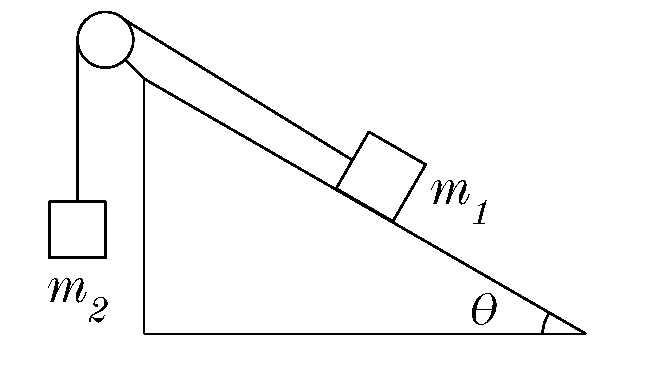
\includegraphics[width = \marginparwidth]{figures/carrucolainclinata.pdf}
    \caption{Piano inclinato molto interessante}
    \label{primo}
\end{marginfigure}
\\\\
\noindent Soluzione:

\section{Tensione delle corde}